\documentclass[11pt,a4paper]{article}
\usepackage[margin=2.2cm]{geometry}
\usepackage{amsmath,booktabs,graphicx,float}
\title{Asymptotic Properties of Estimators:\\ A Simulation Study of the Gamma Model, MLE vs. Method of Moments}
\author{Vitor Dias Ferreira\\ICMC, University of S\~ao Paulo}
\date{Statistical Inference course, 2026}
\begin{document}
\maketitle
\section{Introduction}
This study compares maximum likelihood estimators (MLE) and method-of-moments (MM) estimators of the Gamma distribution. For each sample size $n \in \{20, 50, 100, 200, 500\}$, the R script draws $R = 10{,}000$ Monte Carlo samples with true shape $\alpha_0 = 2$ and true scale $\beta_0 = 3$, and it builds 95\% Wald intervals for both parameters.

\section{Methods}
MM estimators have a closed form: $\hat\alpha = \bar X^2 / S^2$ and $\hat\beta = S^2 / \bar X$. The MLE of $\alpha$ solves a nonlinear equation, handled with Newton--Raphson on the log scale ($\eta = \ln\alpha$) and started at the MM estimate. Then $\hat\beta = \bar X / \hat\alpha$.

Standard errors come from expected Fisher information (MLE-IF), observed information (MLE-IO), and the delta method (MM).

\subsection{Correction to the MM covariance matrix}
The assignment states the MM asymptotic covariance as
\[
\Sigma_{\text{assignment}} = \begin{pmatrix} \alpha(2+\alpha) & \beta(2+\alpha) \\ \beta(2+\alpha) & \beta^2(2+\alpha)/\alpha \end{pmatrix}.
\]
Applying the delta method to $(\bar X, S^2)$, with $\operatorname{Var}(X) = \alpha\beta^2$, $\mu_3 = 2\alpha\beta^3$, and $\mu_4 - \sigma^4 = 2\alpha(\alpha+3)\beta^4$, gives instead
\[
\Sigma_{\text{MM}} = \begin{pmatrix} 2\alpha(\alpha+1) & -2\beta(\alpha+1) \\ -2\beta(\alpha+1) & \beta^2(2\alpha+3)/\alpha \end{pmatrix}.
\]
This study uses $\Sigma_{\text{MM}}$. The change affects only the MM standard errors, interval widths, and coverage. Estimates, bias, and MSE are identical to the earlier run because the seed and the random draws are unchanged.

The empirical standard deviations support the correction. At $n = 500$, the SD of $\hat\alpha_{\text{MM}}$ is 0.155. The corrected formula gives a mean standard error of 0.156, while the assignment's matrix gave 0.127. For $\hat\beta_{\text{MM}}$, the SD is 0.248, against 0.251 (corrected) and 0.189 (assignment). Coverage at $n = 500$ rises from 0.896 to 0.951 for $\alpha$ and from 0.860 to 0.947 for $\beta$.

\section{Results}
\begin{table}[H]
\centering\footnotesize
\caption{Monte Carlo results. MLE-IF and MLE-IO coincide, so the table shows one MLE row. $\alpha_1$: share of intervals entirely above $\theta_0$. $\alpha_2$: share entirely below $\theta_0$.}
\begin{tabular}{rllrrrrrrrrr}
\toprule
$n$ & Par. & Method & Mean & Bias & MSE & SD & Mean SE & Width & Coverage & $\alpha_1$ & $\alpha_2$ \\
\midrule
20 & $\alpha$ & MM & 2.455 & 0.455 & 1.068 & 0.928 & 0.920 & 3.605 & 0.975 & 0.006 & 0.019 \\
20 & $\alpha$ & MLE & 2.309 & 0.309 & 0.719 & 0.790 & 0.685 & 2.684 & 0.961 & 0.010 & 0.030 \\
\addlinespace[2pt]
20 & $\beta$ & MM & 2.785 & -0.215 & 1.342 & 1.139 & 1.176 & 4.609 & 0.852 & 0.000 & 0.148 \\
20 & $\beta$ & MLE & 2.862 & -0.138 & 0.961 & 0.970 & 0.958 & 3.754 & 0.867 & 0.000 & 0.133 \\
\addlinespace[2pt]
50 & $\alpha$ & MM & 2.181 & 0.181 & 0.296 & 0.514 & 0.526 & 2.063 & 0.966 & 0.011 & 0.023 \\
50 & $\alpha$ & MLE & 2.114 & 0.114 & 0.182 & 0.411 & 0.394 & 1.545 & 0.958 & 0.015 & 0.027 \\
\addlinespace[2pt]
50 & $\beta$ & MM & 2.909 & -0.091 & 0.593 & 0.765 & 0.773 & 3.029 & 0.906 & 0.000 & 0.094 \\
50 & $\beta$ & MLE & 2.943 & -0.057 & 0.393 & 0.624 & 0.622 & 2.437 & 0.915 & 0.001 & 0.083 \\
\addlinespace[2pt]
100 & $\alpha$ & MM & 2.089 & 0.089 & 0.131 & 0.351 & 0.359 & 1.408 & 0.957 & 0.018 & 0.025 \\
100 & $\alpha$ & MLE & 2.054 & 0.054 & 0.080 & 0.277 & 0.270 & 1.060 & 0.952 & 0.019 & 0.029 \\
\addlinespace[2pt]
100 & $\beta$ & MM & 2.954 & -0.046 & 0.300 & 0.546 & 0.554 & 2.171 & 0.929 & 0.002 & 0.069 \\
100 & $\beta$ & MLE & 2.972 & -0.028 & 0.200 & 0.447 & 0.444 & 1.739 & 0.930 & 0.005 & 0.065 \\
\addlinespace[2pt]
200 & $\alpha$ & MM & 2.048 & 0.048 & 0.063 & 0.247 & 0.250 & 0.979 & 0.955 & 0.017 & 0.028 \\
200 & $\alpha$ & MLE & 2.029 & 0.029 & 0.037 & 0.190 & 0.189 & 0.739 & 0.954 & 0.022 & 0.024 \\
\addlinespace[2pt]
200 & $\beta$ & MM & 2.973 & -0.027 & 0.155 & 0.392 & 0.394 & 1.543 & 0.941 & 0.005 & 0.054 \\
200 & $\beta$ & MLE & 2.983 & -0.017 & 0.099 & 0.314 & 0.315 & 1.234 & 0.943 & 0.007 & 0.050 \\
\addlinespace[2pt]
500 & $\alpha$ & MM & 2.017 & 0.017 & 0.024 & 0.155 & 0.156 & 0.612 & 0.951 & 0.022 & 0.027 \\
500 & $\alpha$ & MLE & 2.010 & 0.010 & 0.014 & 0.119 & 0.118 & 0.463 & 0.949 & 0.025 & 0.026 \\
\addlinespace[2pt]
500 & $\beta$ & MM & 2.993 & -0.007 & 0.062 & 0.248 & 0.251 & 0.982 & 0.947 & 0.010 & 0.043 \\
500 & $\beta$ & MLE & 2.996 & -0.004 & 0.040 & 0.199 & 0.200 & 0.784 & 0.948 & 0.012 & 0.040 \\
\bottomrule
\end{tabular}
\end{table}

\begin{figure}[H]\centering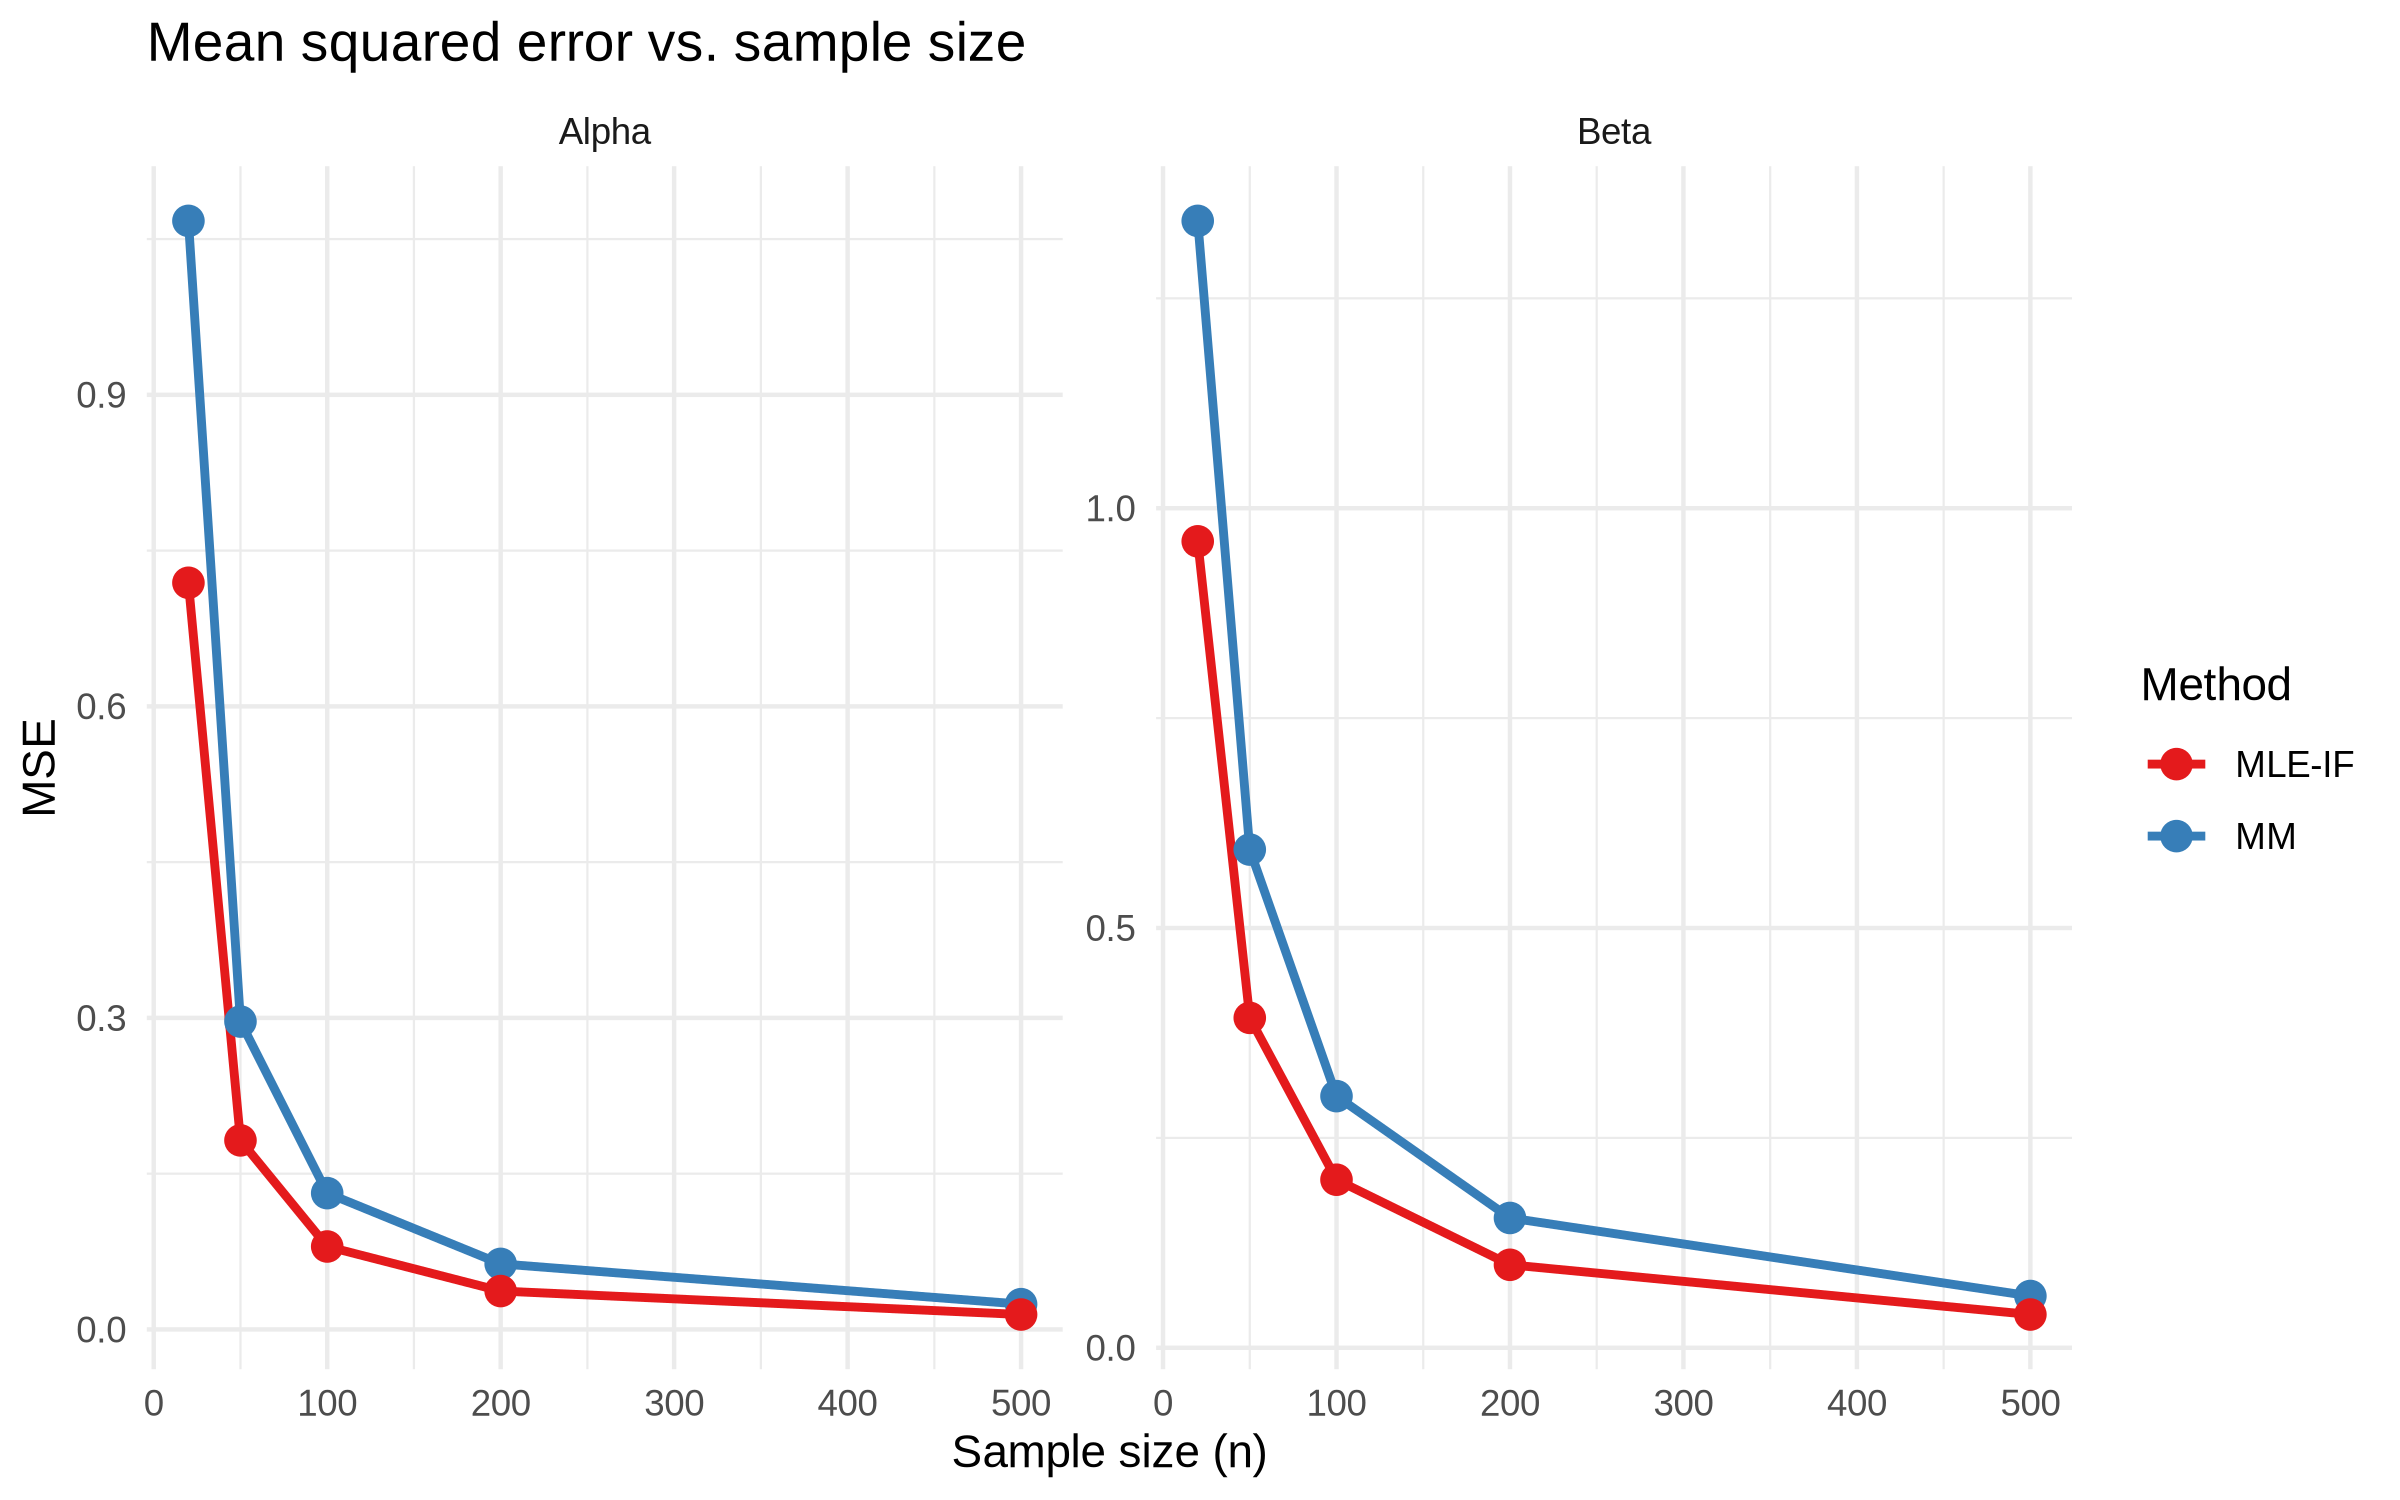
\includegraphics[width=.8\textwidth]{../results/mse.png}\caption{Mean squared error by sample size.}\end{figure}
\begin{figure}[H]\centering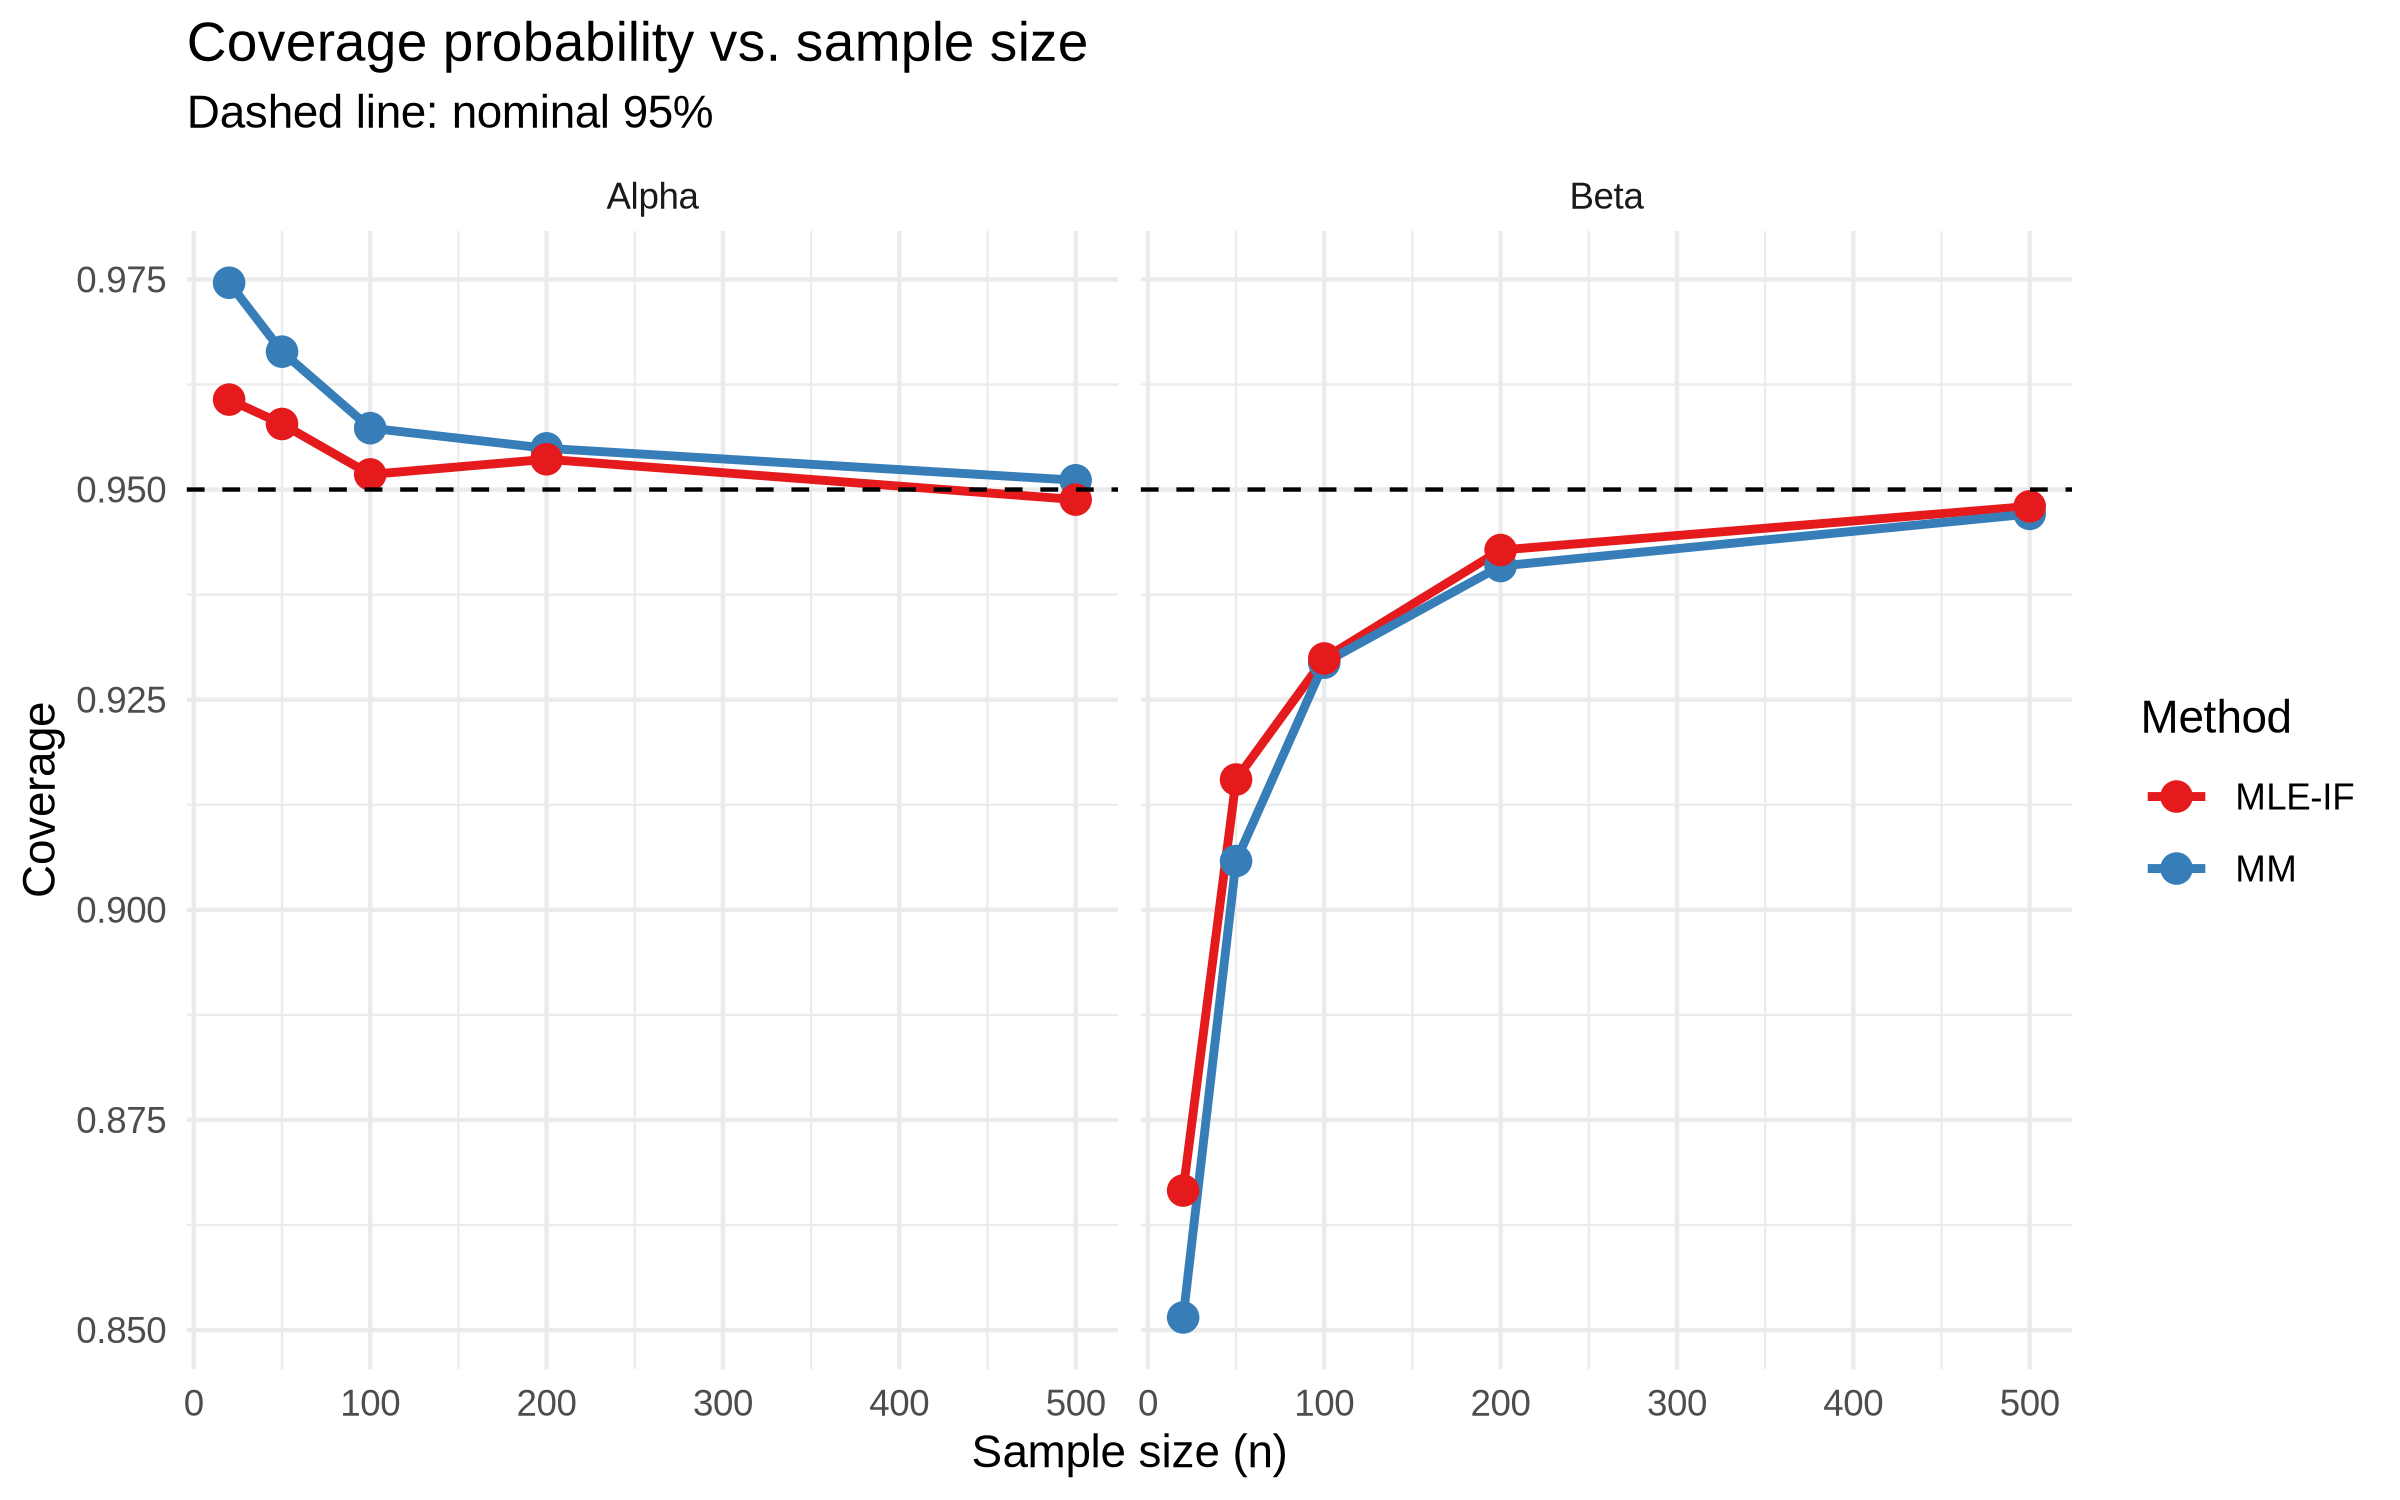
\includegraphics[width=.8\textwidth]{../results/coverage.png}\caption{Coverage by sample size. The dashed line marks the nominal 95\%.}\end{figure}
\begin{figure}[H]\centering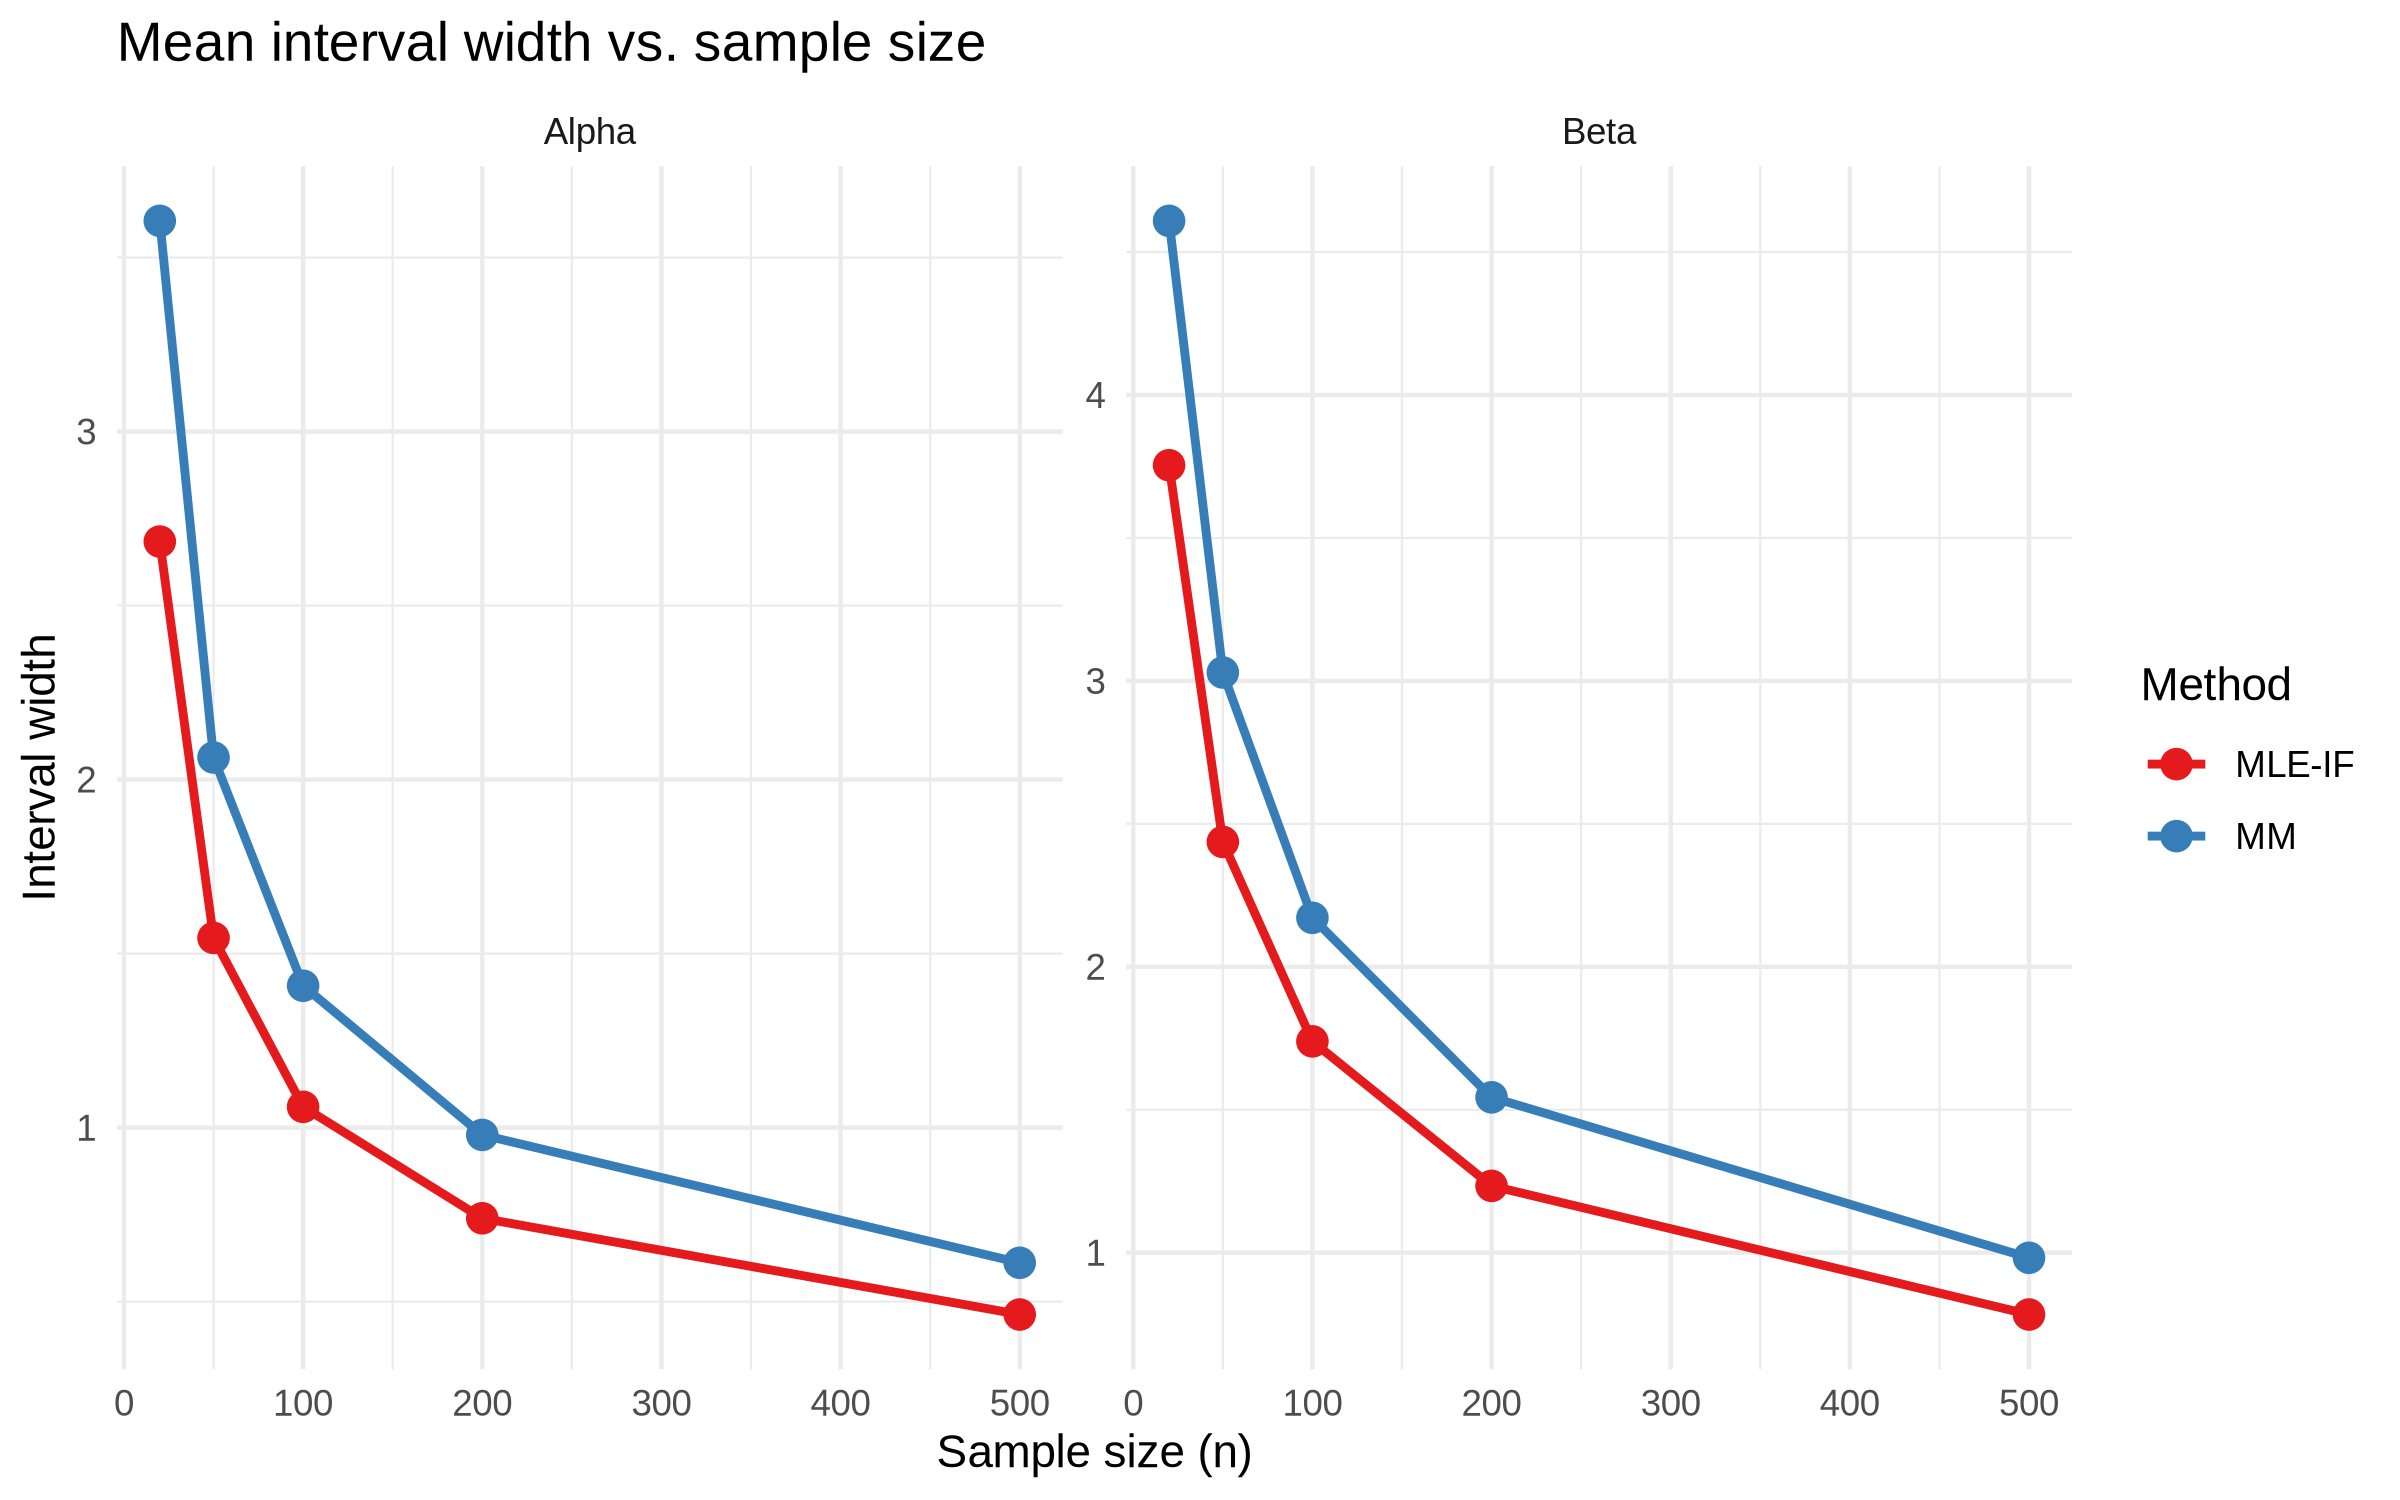
\includegraphics[width=.8\textwidth]{../results/width.png}\caption{Mean interval width by sample size.}\end{figure}

\section{Discussion}
\subsection{Relative efficiency}
MLE has lower MSE than MM at every sample size and for both parameters. At $n = 500$, the MM-to-MLE MSE ratio is 1.69 for $\alpha$ and 1.56 for $\beta$. MM uses only the first two sample moments, whereas the MLE uses the sufficient statistics $\bar X$ and $\overline{\ln X}$, so MM loses information. MM can still be useful where a closed form matters, or as a starting value for iterative methods, as in this implementation.

\subsection{Tails and the normal approximation}
Coverage is unreliable at small $n$. At $n = 20$, intervals for $\beta$ cover only 0.852 (MM) and 0.867 (MLE), and almost all misses are on one side: the interval lies below $\beta_0$. This matches the downward bias of $\hat\beta$ and the skewness of its sampling distribution. Intervals for $\alpha$ at $n = 20$ overcover (0.975 for MM, 0.961 for MLE). By $n = 500$, all methods are within 0.3 percentage points of 95\%, although the misses for $\beta$ remain somewhat unbalanced (0.010 vs. 0.043 for MM).

\subsection{Interval width}
MLE intervals are narrower than corrected MM intervals at all sample sizes, in line with the MLE's lower variance. The earlier results suggested the opposite for $\beta$ only because the assignment's matrix understated MM standard errors.

\subsection{Observed vs. expected information}
MLE-IF and MLE-IO give identical results. This is an algebraic property of the Gamma MLE, not a simulation finding: at the MLE, $\sum_i x_i = n\hat\alpha\hat\beta$, so the observed information equals the expected information evaluated at the estimates.

\section{Conclusion}
MLE dominates MM in efficiency in this setting. Once the MM covariance matrix is corrected, both methods reach nominal coverage at large $n$, and the normal approximation is weak mainly for $\beta$ at small $n$. Results apply to $\alpha_0 = 2$, $\beta_0 = 3$; other parameter values were not studied.
\end{document}
